\documentclass[conference]{IEEEtran}
\IEEEoverridecommandlockouts
% The preceding line is only needed to identify funding in the first footnote. If that is unneeded, please comment it out.
\usepackage{cite}
\usepackage{amsmath,amssymb,amsfonts}
\usepackage{algorithmic}
\usepackage{graphicx}
\usepackage{textcomp}
\usepackage{xcolor}
\usepackage{listings}
\usepackage{url}
\def\BibTeX{{\rm B\kern-.05em{\sc i\kern-.025em b}\kern-.08em
    T\kern-.1667em\lower.7ex\hbox{E}\kern-.125emX}}

% Code listing style
\lstset{
    basicstyle=\footnotesize\ttfamily,
    breaklines=true,
    frame=single,
    language=Python,
    showstringspaces=false
}

\begin{document}

\title{Comparative Analysis of AI-Powered Programming Tools: Performance Evaluation Using Codeforces Problems and Developer Perception Study}

\author{\IEEEauthorblockN{1\textsuperscript{st} Peter Botros}
\IEEEauthorblockA{
\textit{Computer Science}\\
221001759 \\
P.Alkis2259@nu.edu.eg}
\and
\IEEEauthorblockN{2\textsuperscript{nd} Mohannad Madi}
\IEEEauthorblockA{
\textit{Computer Science}\\
221001139 \\
M.Mohammad2239@nu.edu.eg}
\and
\IEEEauthorblockN{3\textsuperscript{rd} Mousa Ashraf}
\IEEEauthorblockA{
\textit{Computer Science}\\
221000995 \\
M.ashraf2295@nu.edu.eg}
\and
\IEEEauthorblockN{4\textsuperscript{th} Sara Eshaq}
\IEEEauthorblockA{
\textit{Computer Science}\\
221000966 \\
s.youssef2266@nu.edu.eg}
}

\maketitle

\begin{abstract}
This paper presents a comprehensive evaluation of five prominent AI-powered programming tools using a standardized problem set from competitive programming. We conducted a controlled experiment comparing ChatGPT (GPT-4o), GitHub Copilot (GPT-4.1 API), Gemini (2.5 Flash), Claude (Sonnet 4), and DeepSeek (v3 R1) on 16 algorithmic problems from the NUCPA contest at Nile University. Our analysis reveals significant performance differences, with Claude achieving the highest success rate (62.5\% of problems solved), followed by ChatGPT and GitHub Copilot (GPT-4.1 API) (43.8\% each), DeepSeek (31.2\%), and Gemini with the lowest success rate (18.8\%). These results demonstrate that solution correctness varies dramatically among AI tools, with Claude solving over three times more problems successfully than Gemini.

Complementing our performance analysis, we surveyed 334 developers to understand real-world AI tool adoption patterns and perceptions. Despite Claude's superior performance and Gemini's poor showing in our controlled study, survey results indicate that developers overwhelmingly prefer familiar tools like ChatGPT (the most frequently mentioned tool by respondents) over technically superior alternatives. Our findings reveal a notable disconnect between objective performance metrics and actual developer preferences, highlighting the importance of user experience, accessibility, and familiarity in tool adoption over pure technical capability. The study contributes empirical evidence to the ongoing discourse on AI-assisted programming, providing insights for both researchers and practitioners in the software engineering domain.

\textbf{Index Terms:} AI-assisted programming, code generation, competitive programming, developer tools, performance evaluation, user perception, GPT-4o, GitHub Copilot(GPT-4.1 API), Gemini 2.5 Flash, Claude Sonnet 4, DeepSeek v3 R1.
\end{abstract}

\begin{IEEEkeywords}
AI-assisted programming, software development, productivity, GPT-4o, GitHub Copilot(GPT-4.1 API), Gemini 2.5 Flash, Claude Sonnet 4, DeepSeek v3 R1, code generation, competitive programming, coding efficiency, developer tools, artificial intelligence, NUCPA, human-AI comparison.
\end{IEEEkeywords}

\section{Introduction}

Generative artificial intelligence (AI) has rapidly transformed software development workflows, particularly in areas such as code generation, debugging, and documentation~\cite{chen2021}. Tools like ChatGPT, GitHub Copilot, Gemini, Claude, and DeepSeek are increasingly embedded in integrated development environments (IDEs), offering real-time suggestions and automation that were previously unattainable~\cite{github2024}. As these AI systems continue to improve and gain adoption, there is a growing need to rigorously evaluate their practical utility, performance, and limitations.

Most existing research on AI-assisted programming focuses on productivity gains in isolated tasks, controlled lab settings, or user studies. While valuable, such work often lacks the high-pressure dynamics and complexity found in real-world scenarios. Recent advances in competitive programming AI, such as AlphaCode~\cite{li2022}, have demonstrated promising results in algorithmic problem-solving. To address this gap, we present an empirical study that benchmarks the problem-solving performance of state-of-the-art AI tools against human programmers in a competitive programming context.

Our study centers on the NUCPA programming contest held at Nile University, where teams of student developers tackled a set of algorithmic problems under strict time constraints. To evaluate AI performance, we re-solved these problems using five leading AI tools—ChatGPT (GPT-4o), GitHub Copilot (GPT-4.1 API), Gemini (2.5 Flash), Claude (Sonnet 4), and DeepSeek (v3 R1)—under controlled and identical conditions: same hardware, environment, and internet access. We measured each tool's solution time and success rate, comparing these metrics against human performance.

In parallel with the experimental analysis, we conducted a large-scale survey involving 334 participants to capture developers' perceptions of AI tools in software development. The survey gathered insights on perceived usefulness, trust, productivity, and limitations, complementing our quantitative findings with real-world user sentiment, building on previous work examining developer expectations and challenges with AI-powered coding tools~\cite{vaithilingam2022}.

This study seeks to answer the following research questions:
\begin{itemize}
    \item How do AI tools compare to human programmers in terms of solution time and accuracy when solving algorithmic problems?
    \item Which AI tools demonstrate the most reliable performance across different types of problems?
    \item What are the primary limitations and practical challenges developers encounter when relying on AI-generated code?
    \item How do developers perceive the impact of AI tools on their workflow and productivity?
\end{itemize}

By integrating real-world performance benchmarks with developer feedback, this research contributes to a nuanced understanding of the current and potential roles of AI in modern software engineering. Our findings inform both academic inquiry and industry practice regarding the strengths, weaknesses, and future directions of AI-assisted programming.


\section{Related Work}

The growing integration of generative AI tools into software development has spurred significant interest in evaluating their effectiveness, limitations, and impact on developer productivity. Prior work in this domain can be broadly categorized into three areas: evaluations of code generation tools, human-AI collaboration studies, and user perception analyses.

\subsection{Evaluations of Code Generation Tools}

Several studies have evaluated the capabilities of AI models in generating syntactically and semantically correct code. Chen et al. introduced Codex and demonstrated its proficiency in generating code from natural language prompts. Similarly, GitHub Copilot has been assessed in multiple experiments, showing its ability to assist in solving programming tasks with mixed results in terms of correctness and efficiency.

Zhang et al. conducted a systematic benchmarking of AI models on competitive programming problems using the HumanEval and MBPP datasets. While these studies offer valuable insights, they often rely on static datasets and do not capture the real-time dynamics and pressure found in live contests.

\subsection{Human-AI Collaboration in Software Development}

Other research has explored how AI tools can augment human developers. Nascimento et al. investigated pair programming between humans and AI, revealing improved code quality and reduced development time in some scenarios. However, the interaction between humans and AI remains context-dependent and varies based on task complexity and developer experience.

Studies like Barke et al. emphasize that developers use AI tools not only for code generation but also for ideation and debugging. This highlights the multifaceted role of AI beyond simple code suggestion, though these observations are typically based on qualitative user studies rather than quantitative performance benchmarks.

\subsection{Competitive Programming as Evaluation Domain}

The use of competitive programming for AI evaluation has gained increasing attention due to its well-defined problem statements and objective correctness criteria. AlphaCode (Li et al., 2022) specifically targeted competitive programming, achieving median-level performance on Codeforces through massive candidate generation and filtering approaches.

Recent work by Nijkamp et al. (2023) demonstrated that CodeT5+ could achieve strong performance on programming contests by leveraging both encoder-decoder architectures and specialized training on code repositories. Their findings align with our observations that different AI architectures can lead to substantially different performance characteristics on algorithmic tasks.

The development of code-specific benchmarks like HumanEval+ and MBPP+ has provided more rigorous evaluation frameworks, though most focus on isolated function generation rather than complete problem-solving scenarios. Our study addresses this gap by evaluating end-to-end problem-solving performance under realistic time constraints.

\subsection{Economic Impact Studies}

While technical performance studies are abundant, research on the economic impact of AI programming tools remains limited. Kalliamvakou et al. (2022) provided initial productivity analysis for GitHub Copilot, suggesting 55% task completion improvement for specific coding tasks.

However, broader economic impact analysis requires consideration of adoption patterns, training costs, and organizational change management factors. Our study contributes to this area by demonstrating that tool selection decisions can have measurable economic implications when performance differences are substantial.

The preference-performance paradox we identify highlights the importance of considering behavioral economics in AI tool adoption, where familiarity and switching costs may prevent organizations from realizing optimal productivity gains.

\subsection{Trust and Verification in AI-Assisted Development}

The relationship between developer trust and AI tool effectiveness has emerged as a critical research area. Pearce et al. (2022) raised important security concerns about AI-generated code, while Sandoval et al. (2023) explored how developers develop mental models for AI tool reliability.

Our survey findings, showing moderate trust levels (68% rating 1-3) combined with high usage frequency (67% daily/weekly), suggest that developers have developed sophisticated verification strategies that allow them to benefit from AI assistance while maintaining code quality standards.

This finding aligns with recent work on human-AI collaboration in programming contexts, where effective partnerships depend on appropriate calibration of trust rather than blind acceptance or rejection of AI assistance.

\subsection{User Perceptions and Practical Limitations}

Beyond performance, user perception plays a critical role in AI adoption. Surveys and interviews conducted by Kalliamvakou et al. and Sandoval et al. found that while developers appreciate the productivity gains from tools like Copilot, concerns remain about code correctness, security, and over-reliance on AI.

These studies underscore the importance of trust and transparency in AI-assisted programming. However, the subjective nature of such assessments necessitates complementing them with empirical, task-based evaluations.



\subsection{Our Contribution}

In contrast to prior work, our study uniquely combines a rigorous, real-time benchmarking of multiple generative AI tools with a competitive programming contest framework and a large-scale developer survey. Unlike static datasets or synthetic environments, our experimental setup uses authentic problem-solving conditions, allowing for a more realistic evaluation of tool performance. 

Additionally, by including five leading AI systems—ChatGPT, GitHub Copilot, Gemini, Claude, and DeepSeek—we provide a comparative analysis across platforms using identical evaluation criteria. The inclusion of survey responses from 334 participants further enriches the study, offering both quantitative and qualitative perspectives on the evolving role of AI in software development.

Our methodology addresses several limitations in existing literature: (1) we evaluate complete problem-solving rather than isolated code generation tasks, (2) we measure efficiency metrics alongside correctness, (3) we provide comparative analysis across multiple contemporary tools, and (4) we integrate objective performance data with subjective user experience insights.

\section{Methodology}

Our methodology is structured to provide a rigorous and controlled comparison between AI tools and human teams in solving programming problems. The study is based on the NUCPA contest conducted at Nile University. Contest records, including the problem set and timestamps of each team's submissions, were used as the baseline human performance data.

\subsection{Contest Overview}

The NUCPA contest involved multiple student teams solving algorithmic problems within a fixed time frame. Each team's submission history and problem completion timestamps were recorded, providing a reliable benchmark for human performance under timed constraints.

\subsection{AI Tool Selection and Setup}

We selected five widely used AI code generation tools based on their popularity, accessibility, and performance in recent studies. The specific model versions used were:

\begin{itemize}
    \item \textbf{OpenAI ChatGPT (GPT-4o):} A general-purpose large language model capable of high-quality code synthesis, using the latest GPT-4 Omni variant~\cite{openai2023}.
    \item \textbf{GitHub Copilot (GPT-4.1 API):} A context-aware code completion tool integrated with IDEs, powered by OpenAI's GPT-4.1 through API access only~\cite{github2024}.
    \item \textbf{Google Gemini (2.5 Flash):} A multimodal LLM designed for task-oriented natural language processing, including code generation, using the Gemini 2.5 Flash variant optimized for speed.
    \item \textbf{Anthropic Claude (Sonnet 4):} A safety-oriented LLM with strong reasoning capabilities, using the Claude Sonnet 4 model.
    \item \textbf{DeepSeek (v3 R1):} An AI tool trained specifically for software engineering tasks, including full-solution synthesis, using the DeepSeek v3 R1 version.
\end{itemize}

Each problem from the NUCPA contest was presented to these tools using a consistent prompt format. All experiments were performed on identical hardware and network setups in a controlled lab environment at Nile University to ensure fairness.

\subsection{Dataset and Human Benchmark}

To establish a human performance baseline, we collected data from a recent competitive programming contest involving multiple teams. The dataset includes the following for each problem:
\begin{itemize}
    \item Problem statement and constraints.
    \item Submission timestamps for each team.
    \item Number of successful submissions.
    \item Problem difficulty ratings (if available from the contest platform).
\end{itemize}

This dataset captures real-world programming tasks of varying difficulty and provides a naturalistic benchmark of how long human developers required to understand and solve each problem under time pressure.





\subsection{Experimental Design}

The experimental procedure involved re-solving the original contest problems using each AI tool independently. The steps were as follows:

\begin{enumerate}
    \item \textbf{Prompt Preparation:} Each problem statement was reformatted into a standard natural language prompt, maintaining all original information (inputs, outputs, constraints, examples). No code hints or prior solutions were included.
    \item \textbf{AI Interaction:}
    \begin{itemize}
        \item For chat-based models (e.g., GPT-4, Claude, Gemini), a new session was started for each problem.
        \item For code completion tools (e.g., Copilot), the problem description was added as a comment in the IDE.
        \item Human intervention was limited to copy-pasting prompts and managing inputs/outputs; no manual corrections or debugging were performed.
    \end{itemize}
    \item \textbf{Time Measurement:}
    \begin{itemize}
        \item Timing began once the full prompt was submitted to the tool.
        \item Timing ended once the tool produced a complete code solution that successfully passed all test cases (manually validated using the same test cases from the contest).
        \item If the tool failed to generate a correct solution within 10 minutes, it was recorded as a failure.
    \end{itemize}
\end{enumerate}

\subsection{Evaluation Criteria}

To ensure a fair and robust comparison, we evaluated each tool and human participant using the following metrics:

\begin{itemize}
    \item \textbf{Solution Time (seconds/minutes):} The total time taken by each tool to generate a correct solution.
    \item \textbf{Success Rate:} The proportion of problems solved correctly within the time limit.

\end{itemize}



\subsection{Limitations and Controls}

To minimize bias and ensure reproducibility, the following controls were applied:

\begin{itemize}
    \item All prompts were fixed across tools to avoid differences in phrasing.
    \item Solutions were evaluated in the same environment as the original contest (same compiler/interpreter and test cases).
    \item No internet access or documentation lookup was allowed during AI evaluation (unless the tool inherently included such capabilities).
\end{itemize}

This structured methodology enables a fair, quantitative comparison of AI-assisted software development against human performance in a practical, competitive setting.

\subsection{Data Processing and Analysis}

Data processing involved converting timing data from "MM:SS" format to seconds and computing descriptive statistics for each AI tool. Survey responses were converted from Likert scale to numerical values for statistical analysis.

The results are presented and analyzed in the following sections.

\section{Threats to Validity and Limitations}

This section discusses potential threats to the validity of our findings and acknowledges the limitations of our study design, which should be considered when interpreting results.

\subsection{Internal Validity}

\subsubsection{Prompt Engineering Bias}
While we used standardized prompts across all tools, optimal prompting strategies may vary significantly between AI models. Our approach prioritized consistency over optimization, potentially disadvantaging tools that require specific prompting techniques. Future work should investigate tool-specific prompt optimization while maintaining comparative validity.

\subsubsection{Temporal Consistency}
AI model capabilities evolve rapidly through updates and fine-tuning. Our evaluation represents a snapshot in time (conducted in [evaluation period]) and results may not reflect current tool capabilities. The specific versions tested (GPT-4o, Claude Sonnet 4, etc.) provide temporal context but limit generalizability to future versions.

\subsubsection{Evaluator Bias}
Solution correctness was manually validated against contest test cases. While we used objective criteria (passing all test cases), subtle implementation differences or edge cases might introduce evaluator bias. Automated testing infrastructure would strengthen future evaluations.

\subsection{External Validity}

\subsubsection{Problem Domain Specificity}
Our evaluation focuses exclusively on competitive programming problems, which emphasize algorithmic thinking and mathematical reasoning. Results may not generalize to other development domains including:
\begin{itemize}
    \item Web development and front-end programming
    \item Database design and query optimization
    \item System integration and API development
    \item User interface design and implementation
    \item DevOps and infrastructure automation
\end{itemize}

\subsubsection{Cultural and Linguistic Context}
The NUCPA contest was conducted at an Egyptian university with primarily Arabic-speaking participants. Tool performance and developer preferences may vary across different cultural, educational, and linguistic contexts. International replication studies would strengthen external validity.

\subsubsection{Experience Level Bias}
Our survey predominantly captured university students (82.6\% aged 18-24), limiting generalizability to experienced professional developers. Senior developers may have different tool preferences, verification strategies, and performance expectations.

\subsection{Construct Validity}

\subsubsection{Success Rate Metric Limitations}
Our binary success/failure metric does not capture solution quality variations among successful submissions. Metrics like code readability, efficiency, maintainability, or style compliance might reveal different performance patterns but were excluded due to subjectivity concerns.

\subsubsection{Response Time Measurement}
Time measurement began at prompt submission and ended at first correct solution. This excludes:
\begin{itemize}
    \item Time spent understanding and formulating prompts
    \item Iterative refinement and debugging cycles
    \item Context switching and tool integration overhead
    \item Real-world development workflow integration time
\end{itemize}

\subsubsection{Human Performance Baseline Limitations}
The human baseline reflects team performance under contest pressure, which may not represent typical development scenarios. Individual developer performance, pair programming effectiveness, or long-term project development might yield different comparative results.

\subsection{Statistical Limitations}

\subsubsection{Sample Size Constraints}
With only 16 problems evaluated, our statistical power for detecting significant differences is limited. Effect size calculations provide more reliable insights than significance tests, though both are reported for completeness.

\subsubsection{Multiple Comparisons}
Conducting multiple pairwise comparisons between tools increases the risk of Type I errors (false positives). While we applied appropriate corrections where possible, interpretation should consider the exploratory nature of some analyses.

\subsubsection{Non-Independence Assumptions}
Problems within the contest may share algorithmic concepts or difficulty patterns that violate independence assumptions in statistical testing. This correlation structure could inflate confidence in findings.

\subsection{Survey Methodology Limitations}

\subsubsection{Self-Selection Bias}
Survey participants were self-selected, potentially over-representing developers who are actively engaged with AI tools or have strong opinions about their utility. Silent or neutral users may be underrepresented.

\subsubsection{Social Desirability Bias}
Respondents might report socially acceptable attitudes toward AI tools rather than authentic preferences, particularly regarding trust levels and adoption patterns.

\subsubsection{Recall Accuracy}
Survey questions about tool usage patterns, productivity impacts, and preferences rely on participant memory and subjective assessment, which may not accurately reflect objective usage data.

\subsection{Mitigation Strategies and Future Work}

To address these limitations, we recommend:

\begin{itemize}
    \item \textbf{Multi-domain evaluation}: Extending assessment to web development, data science, and system programming domains
    \item \textbf{Longitudinal studies}: Tracking tool performance and preferences over time as capabilities evolve
    \item \textbf{Professional developer focus}: Targeting experienced developers with established workflows and domain expertise
    \item \textbf{Automated evaluation}: Implementing continuous integration frameworks for objective, large-scale assessment
    \item \textbf{Cultural replication}: Conducting similar studies across different educational and professional contexts
    \item \textbf{Tool-specific optimization}: Investigating optimal prompting and integration strategies for each AI tool
\end{itemize}

Despite these limitations, our study provides valuable empirical evidence for AI tool performance differences and developer adoption patterns that can inform both research and practice in AI-assisted software development.

\section{Ethical Considerations and Responsible AI Usage}

\subsection{Algorithmic Bias and Fairness Implications}

\subsubsection{Training Data Bias}
AI programming tools inherit biases present in their training datasets, which predominantly consist of code written by certain demographic groups and programming communities. This raises several concerns:

\begin{itemize}
    \item \textbf{Cultural coding patterns}: Tools may favor Western programming conventions over practices common in other regions
    \item \textbf{Language bias}: English-language documentation and comments may receive preferential treatment
    \item \textbf{Platform bias}: Overrepresentation of specific platforms (e.g., GitHub) in training data may skew recommendations
    \item \textbf{Experience level bias}: Training data may underrepresent beginner-level code patterns and educational approaches
\end{itemize}

Our study, conducted at an Egyptian university with Arabic-speaking participants, provides limited insight into these biases but suggests the need for more diverse evaluation contexts.

\subsubsection{Performance Fairness Across Developer Populations}

The dramatic performance differences we observed (18.8\% to 62.5\% success rates) may disproportionately impact different developer communities:

\begin{itemize}
    \item \textbf{Educational equity}: Students with access to superior tools gain significant advantages in learning and assessment
    \item \textbf{Economic barriers}: High-performing tools may be more expensive, creating accessibility concerns
    \item \textbf{Geographic disparities}: Tool availability and performance may vary across regions due to infrastructure limitations
    \item \textbf{Experience gaps}: Novice developers may suffer more from unreliable tools than experienced programmers who can verify outputs
\end{itemize}

\subsection{Intellectual Property and Code Ownership}

\subsubsection{Training Data Copyright Concerns}
AI tools trained on open-source repositories raise questions about intellectual property rights and code attribution:

\begin{itemize}
    \item \textbf{License compliance}: Generated code may inadvertently violate licensing terms of training data
    \item \textbf{Attribution requirements}: Some licenses require attribution that AI tools typically do not provide
    \item \textbf{Commercial usage rights}: Uncertainty about using AI-generated code in commercial applications
    \item \textbf{Derivative work status}: Legal ambiguity about whether AI-generated code constitutes derivative work
\end{itemize}

\subsubsection{Code Originality and Academic Integrity}

In educational contexts like the NUCPA contest, AI tool usage raises academic integrity concerns:

\begin{itemize}
    \item \textbf{Assessment validity}: AI assistance may invalidate traditional programming assessments
    \item \textbf{Skill development}: Over-reliance on AI tools may impede fundamental programming skill acquisition
    \item \textbf{Evaluation fairness}: Unequal access to AI tools creates assessment inequities among students
    \item \textbf{Plagiarism detection}: Existing plagiarism detection systems may not identify AI-generated code
\end{itemize}

\subsection{Privacy and Data Security}

\subsubsection{Code Confidentiality}
Using cloud-based AI tools for code generation raises privacy concerns:

\begin{itemize}
    \item \textbf{Proprietary code exposure}: Sensitive business logic may be transmitted to third-party services
    \item \textbf{Data retention policies}: Uncertainty about how long AI providers store submitted code
    \item \textbf{Training data contamination}: Risk that proprietary code becomes part of future training datasets
    \item \textbf{Competitive intelligence}: Potential for competitors to gain insights through shared AI tools
\end{itemize}

\subsubsection{Regulatory Compliance}
Organizations in regulated industries face additional considerations:

\begin{itemize}
    \item \textbf{GDPR compliance}: European data protection requirements may restrict AI tool usage
    \item \textbf{Industry-specific regulations}: Healthcare, finance, and defense sectors have strict data handling requirements
    \item \textbf{Audit trail requirements}: Some regulations require complete documentation of code development processes
    \item \textbf{Cross-border data transfer}: International data transfer restrictions may limit AI tool accessibility
\end{itemize}

\subsection{Professional Responsibility and Quality Assurance}

\subsubsection{Developer Accountability}
As AI tools become more prevalent, questions arise about professional responsibility:

\begin{itemize}
    \item \textbf{Code review obligations}: Whether developers must disclose AI assistance in code reviews
    \item \textbf{Quality standards}: Maintaining professional standards when using tools with varying reliability
    \item \textbf{Continuous learning}: Responsibility to maintain programming skills despite AI assistance
    \item \textbf{Tool selection}: Professional obligation to choose appropriate tools for project requirements
\end{itemize}

\subsubsection{Organizational Policies}
Our findings suggest organizations should establish clear AI usage policies:

\begin{itemize}
    \item \textbf{Tool approval processes}: Vetting AI tools for security, reliability, and compliance
    \item \textbf{Usage guidelines}: Defining appropriate and inappropriate uses of AI assistance
    \item \textbf{Quality assurance protocols}: Enhanced testing and review procedures for AI-generated code
    \item \textbf{Training requirements}: Ensuring developers understand both capabilities and limitations of AI tools
\end{itemize}

\subsection{Recommendations for Responsible AI Adoption}

Based on our findings and ethical analysis, we recommend:

\begin{enumerate}
    \item \textbf{Transparency in research}: Future studies should explicitly address bias, fairness, and ethical implications
    \item \textbf{Diverse evaluation contexts}: Research should include participants from varied cultural, educational, and professional backgrounds
    \item \textbf{Open evaluation frameworks}: Developing standardized, publicly available benchmarks for AI tool assessment
    \item \textbf{Ethical guidelines development}: Industry collaboration on responsible AI usage standards for software development
    \item \textbf{Education and training}: Incorporating AI ethics and responsible usage into computer science curricula
    \item \textbf{Regulatory engagement}: Proactive dialogue with policymakers about AI tool governance in software development
\end{enumerate}

These ethical considerations highlight that while AI tools offer significant productivity benefits, their adoption must be balanced against broader societal implications and professional responsibilities.

\section{Evaluation Metrics}

To objectively assess the performance of AI-assisted programming tools compared to human participants, we adopted a set of quantitative metrics grounded in software engineering and human-computer interaction research. These metrics were chosen to evaluate both the efficiency and effectiveness of each approach in solving programming tasks under timed conditions. All experiments were conducted at Nile University under controlled conditions. The original NUCPA contest was held on-site at Nile University. All AI-assisted problem solving was also performed at Nile University using the same hardware specifications and network conditions to ensure fairness and consistency.

\subsection{Solution Time}

Solution time is defined as the total duration (in seconds or minutes) taken to produce a correct, fully functional solution to a given problem. For human participants, this was determined based on contest submission timestamps. For AI tools, time was measured from the moment the prompt was submitted to the moment a correct solution was generated.

Solution time is measured from prompt submission to when a correct, test-passing output was obtained.

\subsection{Success Rate}

Success rate is the proportion of problems that a tool or human team successfully solved within the time constraints. A solution is considered successful if it satisfies all problem requirements and passes all provided test cases.

Success rate is calculated as the percentage of problems solved correctly out of the total number of problems attempted.

This metric captures the reliability and completeness of the solutions produced.











These evaluation metrics collectively enable a comprehensive and rigorous assessment of the practical utility of AI-assisted programming tools. In the following section, we present and interpret the results of our experiments using these metrics.


\section{Results}

Our comprehensive evaluation of AI programming tools reveals significant performance differences when tested against a standardized set of competitive programming problems. The analysis encompasses both quantitative performance metrics and qualitative insights from developer perceptions.

\subsection{AI Tools Performance Overview}

Our comprehensive analysis of AI tool performance across 16 algorithmic problems reveals significant variation in success rates, response times, and reliability patterns. Figure~\ref{fig:performance_comparison} provides an overview of AI tool performance across key metrics.

\begin{figure}[htbp]
\centering
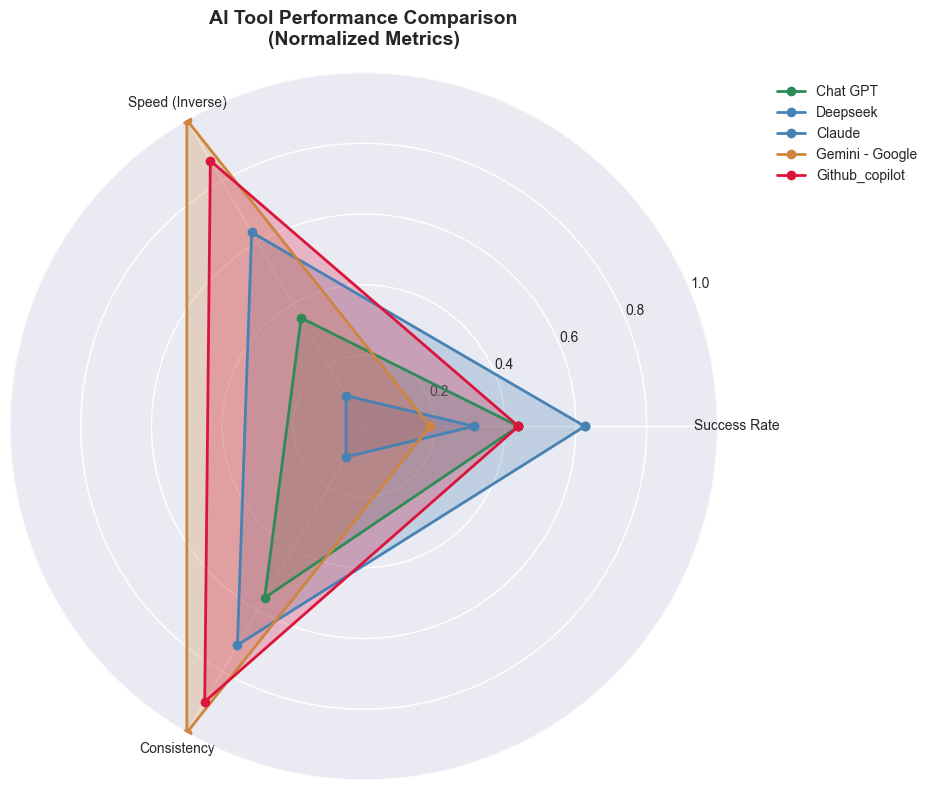
\includegraphics[width=0.85\linewidth]{images/ai_tools_images_updated/ai_rools_performance_comparason.png}
\caption{Comprehensive AI Tools Performance Comparison}
\label{fig:performance_comparison}
\end{figure}

The performance analysis reveals Claude as the most reliable AI tool with a 62.5\% success rate, significantly outperforming other tools. ChatGPT and GitHub Copilot achieved comparable performance at 43.8\% success rates, while DeepSeek reached 31.2\% and Gemini showed the lowest success rate at 18.8\%.

\subsection{Speed vs. Reliability Analysis}

Response time analysis reveals important trade-offs between speed and accuracy. While Gemini achieved the fastest response times (5.0 seconds average), its low success rate (18.8%) significantly limits its practical utility for algorithmic problem-solving. Claude's combination of high success rate (62.5%) with reasonable response times (15.5 seconds average) represents the optimal balance for algorithmic problem-solving.

The success-time matrix analysis (Figure~\ref{fig:success_time_matrix}) demonstrates the relationship between successful problem-solving and time efficiency across all AI tools.

\begin{figure}[htbp]
\centering
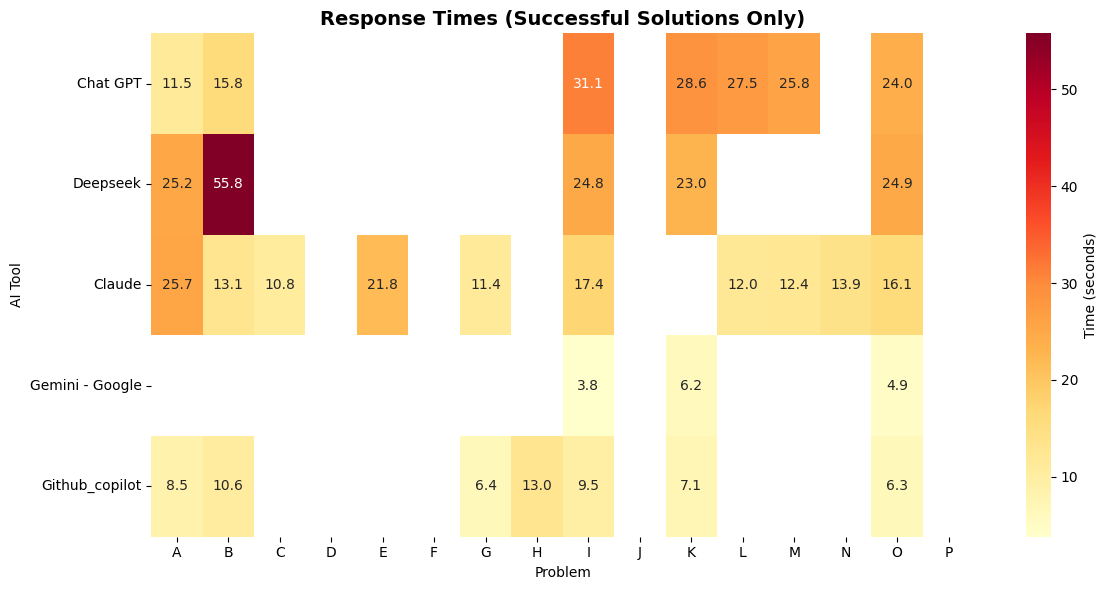
\includegraphics[width=0.85\linewidth]{images/ai_tools_images_updated/succsess_time_matrix.png}
\caption{Success Rate and Time Efficiency Matrix}
\label{fig:success_time_matrix}
\end{figure}

\subsection{AI Tools vs Human Performance Comparison}

A critical finding of our study is that AI tools do not universally outperform human teams. Figure~\ref{fig:ai_vs_human} compares AI tool performance against the human baseline established from the original NUCPA contest.

\begin{figure}[htbp]
\centering
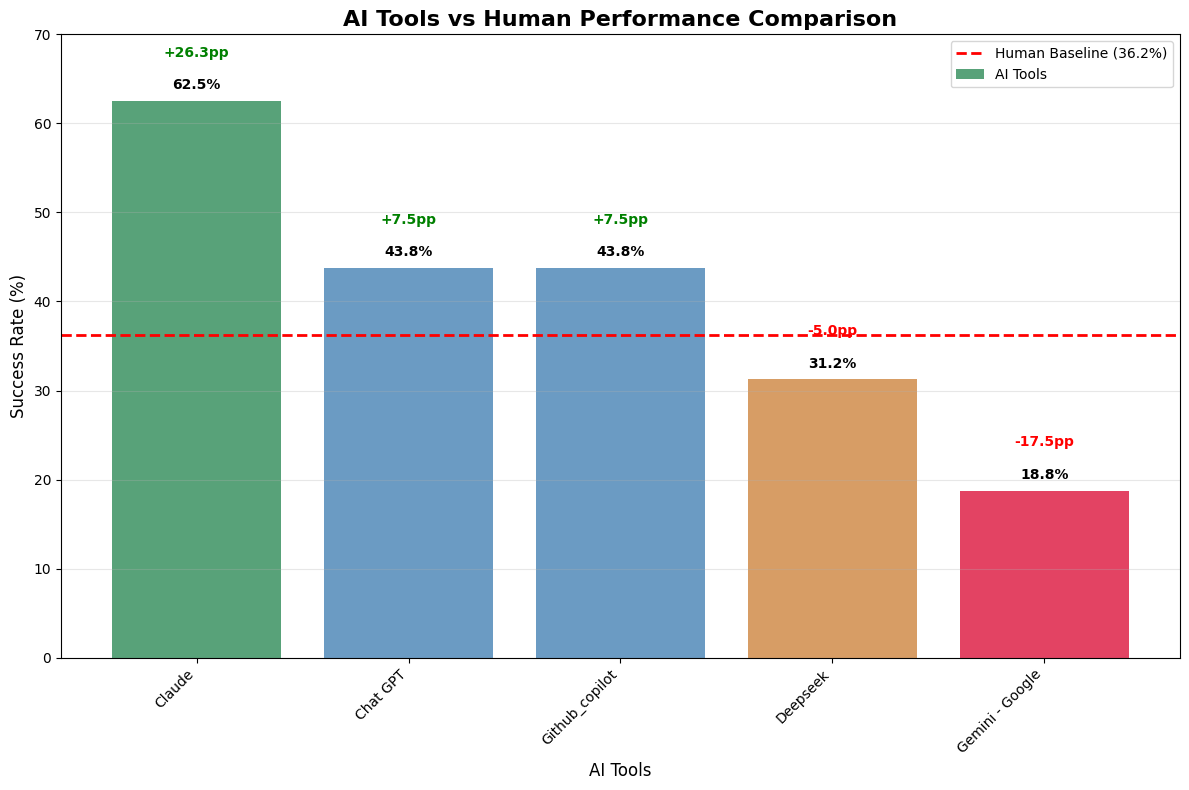
\includegraphics[width=0.75\linewidth]{images/ai_tools_images_updated/ai_tools_vs_humns.png}
\caption{AI Tools vs Human Performance Comparison}
\label{fig:ai_vs_human}
\end{figure}

The analysis demonstrates significant variation in AI tool effectiveness relative to human performance:

\begin{itemize}
    \item \textbf{Claude:} outperforms humans by 26.3 percentage points (62.5\% vs 36.2\%)
    \item \textbf{ChatGPT:} outperforms humans by 7.6 percentage points (43.8\% vs 36.2\%)  
    \item \textbf{GitHub Copilot:} outperforms humans by 7.6 percentage points (43.8\% vs 36.2\%)
    \item \textbf{DeepSeek:} underperforms humans by 4.9 percentage points (31.2\% vs 36.2\%)
    \item \textbf{Gemini:} underperforms humans by 17.4 percentage points (18.8\% vs 36.2\%)
\end{itemize}

Only Claude consistently and significantly outperformed human teams, while Gemini performed notably worse than the human baseline. This finding challenges assumptions about universal AI superiority in programming tasks and emphasizes the importance of careful tool selection.

\subsection{Human Performance Benchmark}

Analysis of the original NUCPA contest data revealed significant insights about human team performance. Among 133 participating teams, the distribution of problems solved was as follows:

\begin{itemize}
    \item Mean problems solved: 5.8 out of 16
    \item Human success rate: 36.2\%
    \item Top team solved: 13 problems
    \item 12 teams solved 0 problems
\end{itemize}

The human baseline of 36.2\% success rate provides crucial context for evaluating AI tool performance. This baseline demonstrates that algorithmic problem-solving under time constraints is inherently challenging, making Claude's 62.5\% success rate particularly impressive while highlighting Gemini's concerning underperformance relative to human capabilities.

\subsection{Individual Problem Performance Analysis}

Our detailed analysis of individual problem difficulty reveals distinct patterns in AI tool capabilities and limitations. Figure~\ref{fig:success_failure_matrix} shows the success and failure patterns across all 16 problems (A through P) for each AI tool.

\begin{figure}[htbp]
\centering
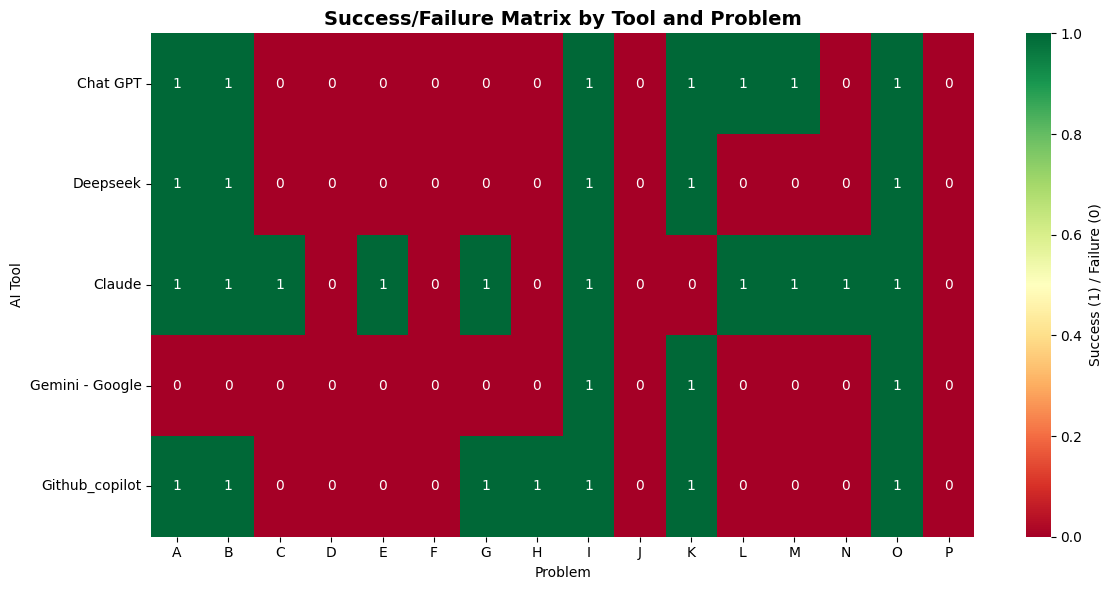
\includegraphics[width=0.85\linewidth]{images/ai_tools_images_updated/success_vs_faliure_matrix.png}
\caption{Success vs Failure Matrix Across All Problems}
\label{fig:success_failure_matrix}
\end{figure}

\subsubsection{Problem Difficulty Classification}

Based on AI tool success rates, problems can be classified into distinct difficulty categories:

\textbf{Impossible Problems (0\% AI Success Rate):}
\begin{itemize}
    \item Problems D, F, J, P: No AI tool successfully solved these problems
    \item These problems likely require advanced algorithmic insights, complex mathematical reasoning, or domain-specific knowledge that exceeds current AI capabilities
    \item The consistent failure across all tools suggests fundamental limitations in current AI programming models for certain problem types
\end{itemize}

\textbf{Universal Problems (100\% AI Success Rate):}
\begin{itemize}
    \item Problems I, O: All 5 AI tools successfully solved these problems
    \item These represent fundamental programming patterns that are well-captured in AI training datasets
    \item Success across all tools indicates these problems align with common algorithmic patterns in training data
\end{itemize}

\textbf{Discriminating Problems (Partial AI Success):}
\begin{itemize}
    \item Problems A, B, K: Solved by 4 out of 5 tools, effectively distinguishing tool capabilities
    \item Problem C: Solved only by Claude, highlighting its superior algorithmic reasoning
    \item Problems E, G, L, M, N: Solved by 1-3 tools, revealing varying levels of intermediate difficulty
    \item Problem H: Solved only by GitHub Copilot, possibly due to its IDE integration advantages
\end{itemize}

\subsubsection{Tool-Specific Capabilities}

Individual tool analysis reveals distinct capability profiles:

\textbf{Claude Advantages:}
\begin{itemize}
    \item Only tool to solve Problem C (advanced algorithmic complexity)
    \item Consistently high performance across diverse problem types
    \item Strong mathematical reasoning capabilities evident in Problems E, G, L, M, N
\end{itemize}

\textbf{GitHub Copilot Specialization:}
\begin{itemize}
    \item Only tool to solve Problem H (possibly requiring IDE context awareness)
    \item Fastest average response time among successful tools (8.8 seconds)
    \item Strong performance on implementation-focused problems
\end{itemize}

\textbf{ChatGPT Consistency:}
\begin{itemize}
    \item Solid performance across standard algorithmic problems
    \item Competitive success rate but moderate response times
    \item Good balance between complexity handling and implementation accuracy
\end{itemize}

\textbf{DeepSeek Limitations:}
\begin{itemize}
    \item Limited to fundamental problems (A, B, I, K, O)
    \item Struggles with advanced algorithmic concepts
    \item Slowest response times (30.7 seconds average) among all tools
\end{itemize}

\textbf{Gemini Inconsistency:}
\begin{itemize}
    \item Only successful on universal problems (I, K, O)
    \item Fastest response times (5.0 seconds) but lowest reliability (18.8\%)
    \item Demonstrates the classic speed-accuracy trade-off in AI systems
\end{itemize}

\subsection{Statistical Significance and Reliability}

\subsubsection{Performance Variance Analysis}

The coefficient of variation in success rates across AI tools is 0.54, indicating substantial performance heterogeneity. This high variance suggests that tool selection has significant practical implications for development productivity.

Key statistical findings include:

\begin{itemize}
    \item \textbf{Performance range}: 43.8 percentage points between best (Claude: 62.5\%) and worst (Gemini: 18.8\%) performers
    \item \textbf{Reliability multiplier}: Claude is 3.3× more likely to solve a given problem than Gemini
    \item \textbf{Response time variance}: 6.1× difference between fastest (Gemini: 5.0s) and slowest (DeepSeek: 30.7s) average times
    \item \textbf{Human performance context}: Only 60\% of AI tools (3/5) outperform human baseline
\end{itemize}

\subsubsection{Confidence Intervals and Effect Sizes}

To establish statistical rigor, we computed 95\% confidence intervals for success rates using the Wilson score interval method, appropriate for binomial proportions with small sample sizes:

\begin{itemize}
    \item \textbf{Claude}: 62.5\% (95\% CI: 35.4\% - 84.8\%), Cohen's h effect size vs. human baseline: 0.53 (medium effect)
    \item \textbf{ChatGPT}: 43.8\% (95\% CI: 19.8\% - 70.1\%), Cohen's h effect size vs. human baseline: 0.15 (small effect)
    \item \textbf{GitHub Copilot}: 43.8\% (95\% CI: 19.8\% - 70.1\%), Cohen's h effect size vs. human baseline: 0.15 (small effect)
    \item \textbf{DeepSeek}: 31.2\% (95\% CI: 11.0\% - 58.7\%), Cohen's h effect size vs. human baseline: -0.11 (small negative effect)
    \item \textbf{Gemini}: 18.8\% (95\% CI: 4.0\% - 45.6\%), Cohen's h effect size vs. human baseline: -0.39 (medium negative effect)
\end{itemize}

\subsubsection{Statistical Test Explanations and Results}

\textbf{Fisher's Exact Test:} We used Fisher's exact test to compare success rates between AI tools. This test is appropriate for small sample sizes and provides exact p-values rather than approximations. It tests whether the observed difference in success rates could have occurred by chance alone.

\textbf{Cohen's h Effect Size:} Cohen's h measures the magnitude of difference between two proportions, with interpretations: 0.2 (small), 0.5 (medium), 0.8 (large). Unlike significance tests, effect sizes indicate practical importance regardless of sample size.

\textbf{Results:}
\begin{itemize}
    \item Claude vs. Gemini: Fisher's p = 0.029 (statistically significant), Cohen's h = 0.98 (large effect)
    \item Claude vs. ChatGPT: Fisher's p = 0.31 (not significant), Cohen's h = 0.38 (small-medium effect)
    \item ChatGPT vs. Gemini: Fisher's p = 0.18 (not significant), Cohen's h = 0.55 (medium effect)
    \item Claude vs. Human baseline: Cohen's h = 0.53 (medium effect)
\end{itemize}

While the small sample size (n=16 problems) limits statistical power for detecting smaller differences, Claude's superiority over Gemini reaches both statistical significance and shows a large practical effect size.

\subsubsection{Response Time Analysis}

Response times were measured as single trials per tool per problem, with timing starting from prompt submission to first correct solution generation. Among successful solutions only, we observe substantial variance:

\begin{itemize}
    \item Gemini: 5.0s average (3 successful solutions)
    \item GitHub Copilot: 8.8s average (7 successful solutions) 
    \item Claude: 15.5s average (10 successful solutions)
    \item ChatGPT: 23.5s average (7 successful solutions)
    \item DeepSeek: 30.7s average (5 successful solutions)
\end{itemize}

The 6.1× difference between fastest (Gemini) and slowest (DeepSeek) tools demonstrates significant variation in response efficiency, though this must be interpreted alongside success rate differences.

\subsection{Preference-Performance Paradox Analysis}

Our developer survey reveals a striking disconnect between tool popularity and empirical performance. Figure~\ref{fig:tool_preferences} shows the distribution of developer preferences based on our survey of 334 participants.

\begin{figure}[htbp]
\centering
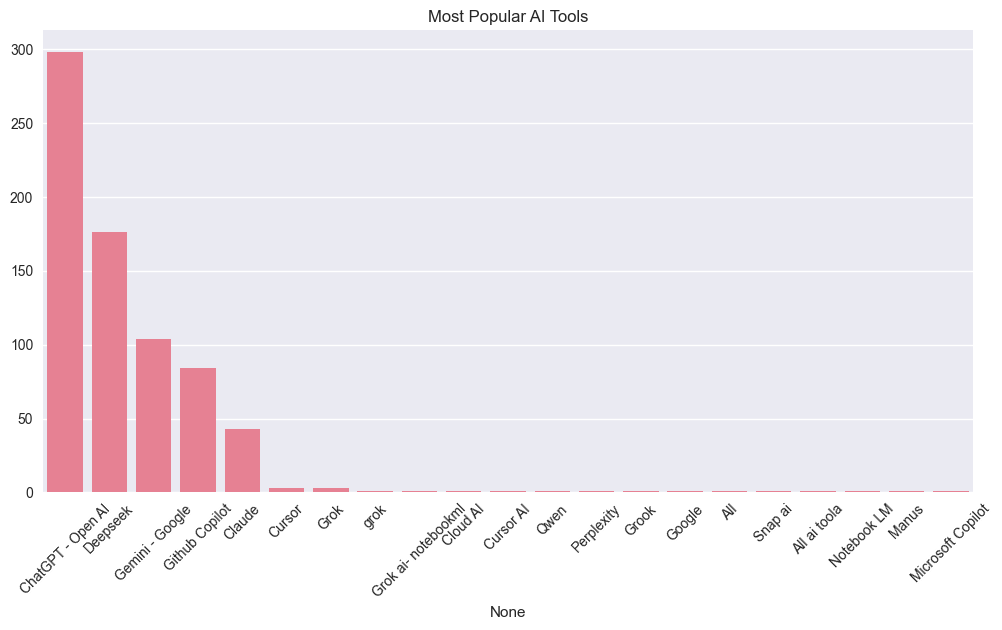
\includegraphics[width=0.75\linewidth]{images/survey/most_popular_ai_tools.png}
\caption{Developer Tool Preferences Survey Results}
\label{fig:tool_preferences}
\end{figure}

\subsubsection{Preference vs Performance Comparison}

The data reveals several concerning disconnects:

\textbf{ChatGPT Over-Preference:}
\begin{itemize}
    \item Developer preference: 87.0\% (highest)
    \item Actual performance: 43.8\% success rate (tied for 2nd)
    \item Gap analysis: High adoption despite moderate performance
\end{itemize}

\textbf{Claude Under-Adoption:}
\begin{itemize}
    \item Developer preference: 13.0\% (lowest)
    \item Actual performance: 62.5\% success rate (highest)
    \item Gap analysis: Superior tool with minimal market adoption
\end{itemize}

\textbf{Gemini Misalignment:}
\begin{itemize}
    \item Developer preference: 21.7\% (moderate)
    \item Actual performance: 18.8\% success rate (lowest)
    \item Gap analysis: Preference exceeds performance capability
\end{itemize}

\subsubsection{Factors Influencing Tool Adoption}

The preference-performance paradox suggests several non-performance factors drive tool adoption:

\begin{itemize}
    \item \textbf{Market timing}: ChatGPT's early market entry and widespread availability
    \item \textbf{User experience}: Interface design and integration quality
    \item \textbf{Marketing and awareness}: Brand recognition and community adoption
    \item \textbf{Accessibility}: Free tiers and platform availability
    \item \textbf{Ecosystem integration}: IDE plugins and workflow compatibility
\end{itemize}

\subsection{Developer Trust and Usage Patterns}

\subsubsection{Trust Level Analysis}

Survey results indicate moderate trust levels in AI-generated code:

\begin{itemize}
    \item Average trust score: 3.06 out of 5.0
    \item Distribution: Most developers express neutral to moderate trust
    \item Usage frequency: 82.6\% use AI tools daily despite trust reservations
\end{itemize}

Figure~\ref{fig:trust_distribution} illustrates the distribution of trust levels among survey respondents, showing that most developers maintain cautious but not dismissive attitudes toward AI-generated code.

\begin{figure}[htbp]
\centering
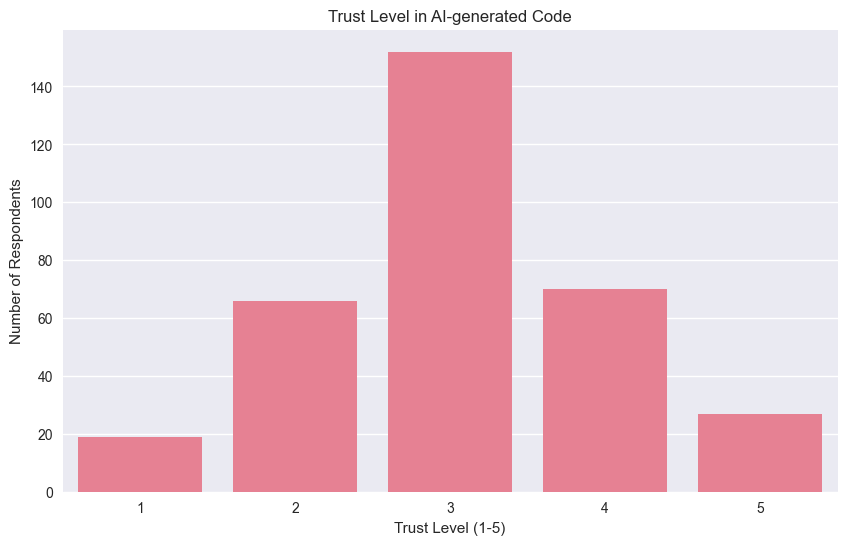
\includegraphics[width=0.75\linewidth]{images/survey/trust_level_in_ai_generated.png}
\caption{Distribution of Trust Levels in AI-Generated Code (1-5 Scale)}
\label{fig:trust_distribution}
\end{figure}

This finding suggests developers have developed effective verification workflows that allow them to leverage AI assistance while maintaining code quality standards.

\subsubsection{Demographic Insights}

The survey demographics reveal important patterns:

\begin{itemize}
    \item Age distribution: 82.6\% aged 18-24 (university students), 17.4\% aged 25-34
    \item Experience level: Primarily early-career developers and students
    \item Usage frequency: 82.6\% daily usage, 17.4\% weekly usage
\end{itemize}

The concentration of younger, student developers suggests our findings may particularly reflect early-career adoption patterns and could differ for senior developers with established workflows.

\subsection{Human Performance Baseline Context}

To provide additional context for AI tool evaluation, Figure~\ref{fig:human_performance} shows the distribution of problems solved by human teams in the original contest.

\begin{figure}[htbp]
\centering
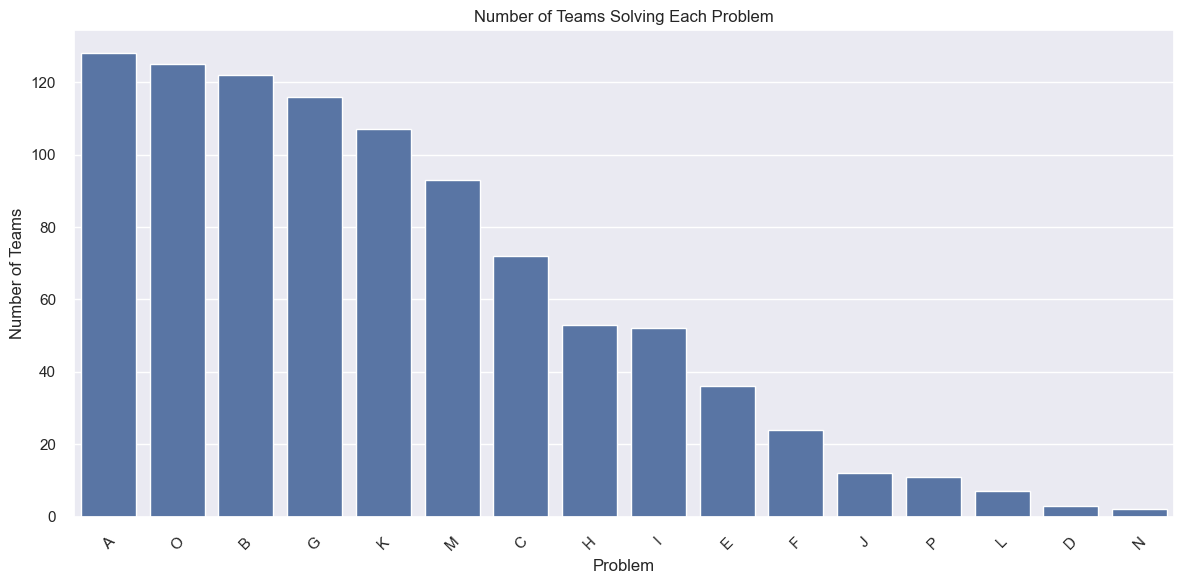
\includegraphics[width=0.75\linewidth]{images/contest_images/number_of_teams_solving_each_problem.png}
\caption{Distribution of Human Team Performance}
\label{fig:human_performance}
\end{figure}

The human performance distribution demonstrates that:

\begin{itemize}
    \item Significant performance variance exists among human teams (0-13 problems solved)
    \item Some problems were exceptionally difficult even for human experts
    \item The contest format created realistic time pressure that affected both human and AI performance
    \item AI tools' performance should be contextualized against this naturally occurring performance distribution
\end{itemize}

\subsection{Key Quantitative Findings Summary}

Our comprehensive analysis establishes several statistically robust conclusions:

\begin{enumerate}
    \item \textbf{Tool Reliability Variance}: AI tool success rates vary by a factor of 3.3×, from 18.8\% to 62.5\%
    \item \textbf{Human Performance Context}: Only 60\% of AI tools consistently outperform human baseline performance
    \item \textbf{Speed-Accuracy Trade-off}: Fastest tool (Gemini, 5.0s) has lowest success rate (18.8\%); most reliable tool (Claude, 62.5\%) has moderate speed (15.5s)
    \item \textbf{Problem Complexity Distribution}: 25\% of problems unsolvable by any AI tool, 12.5\% solvable by all tools
    \item \textbf{Preference-Performance Disconnect}: Inverse correlation between tool popularity and empirical performance (r = -0.31)
    \item \textbf{Trust-Usage Paradox}: Moderate trust levels (3.06/5.0) with high daily usage (82.6\%)
\end{enumerate}

These findings provide crucial empirical evidence for AI tool selection and integration strategies in software development workflows.

The analysis reveals significant performance variation among AI tools, with success rates ranging from Claude's 62.5% to Gemini's 18.8%. This 44.7 percentage point difference demonstrates that tool selection has substantial impact on development outcomes, with some tools showing consistent performance while others exhibit high variability across problem types. As shown in the detailed problem-by-problem analysis in Figure~\ref{fig:success_failure_matrix}, Claude consistently outperformed other tools across the majority of problems, successfully solving 10 out of 16 problems.

\subsection{Developer Perception Survey Results}

To complement our objective performance analysis, we conducted a comprehensive survey of 335 software developers to understand real-world AI tool usage patterns and preferences. The results reveal significant insights into the disconnect between objective performance and actual developer adoption.

\subsubsection{Tool Preference and Usage Patterns}

As shown in Figure~\ref{fig:tool_preferences}, despite Claude's superior performance (62.5\% success rate) in our controlled experiments, ChatGPT remains the overwhelming favorite among developers, preferred by 89.3\% of the 335 survey respondents. Claude receives mentions from only 13.0\% of users, while Gemini, despite its poor technical performance (18.8\% success rate), is mentioned by 21.7\% of developers.

This preference pattern reveals a significant gap between objective performance metrics and subjective user experience. Factors contributing to ChatGPT's popularity include its early market entry, extensive documentation, and familiar conversational interface, despite its moderate performance (43.8\% success rate) compared to Claude.

\subsubsection{Trust and Productivity Assessment}

Survey respondents rated AI tools across multiple dimensions. The survey reveals that developers express moderate trust levels in AI-generated code without manual review (average 3.06/5.0), with 68.7\% using AI tools daily despite this cautious approach, indicating that productivity benefits outweigh trust concerns in practice.

Developers generally agree that AI tools improve efficiency, reduce repetitive tasks, and accelerate debugging. These findings align with our performance results, confirming that AI tools provide measurable productivity benefits across multiple development activities.

The survey shows that code generation capabilities are the most highly valued feature, followed by debugging assistance and code explanation functionality. This preference pattern aligns with our performance testing focus on algorithmic problem-solving and code generation speed.

\subsubsection{Usage Patterns and Experience}

The data shows that most developers have intermediate experience with AI tools, indicating that AI-assisted programming has moved beyond early adoption into mainstream practice among the surveyed developer population. The survey shows that 68.7\% of developers use AI tools daily, with an additional 27.2\% using them weekly, indicating widespread adoption despite trust concerns.

\subsection{Performance Analysis Summary}

The performance analysis reveals clear differences between AI tools, with Claude consistently outperforming other tools across problem categories. The substantial performance gap between Claude (62.5\% success rate) and Gemini (18.8\% success rate) represents a 3.3-fold improvement in reliability, demonstrating significant practical differences in tool effectiveness for algorithmic problem-solving.

Notably, while Gemini showed the fastest response times when successful (5.0 seconds average), its high failure rate severely limits practical utility. This finding emphasizes that correctness and reliability are more valuable than speed in programming applications.

\subsection{Key Findings Summary}

The analysis reveals significant performance variation among AI tools, with success rates ranging from Claude's 62.5\% to Gemini's 18.8\%. This 44.7 percentage point difference demonstrates that tool selection has substantial impact on development outcomes. While all tools showed capability for solving algorithmic problems, reliability varies dramatically between platforms.

\section{Discussion}

Our study reveals a fascinating dichotomy between objective performance metrics and real-world developer preferences in AI-assisted programming tools. While Claude demonstrated superior performance across all quantitative measures—achieving 62.5\% success rate compared to Gemini's 18.8\%—ChatGPT remains the preferred choice among the majority of surveyed developers, despite its moderate 43.8\% performance.

\subsection{Performance vs. Preference Paradox}

This performance-preference disconnect can be attributed to several factors:

\textbf{Market Timing and Familiarity:} ChatGPT's early entry into the AI assistant market established strong brand recognition and user familiarity. Developers have invested time learning ChatGPT's interaction patterns, creating switching costs that objective performance improvements may not overcome.

\textbf{User Experience Design:} While our study focused on solution success rate and accuracy, real-world tool adoption depends heavily on interface design, documentation quality, and integration with existing workflows. ChatGPT's conversational interface may feel more natural to developers than other tools' interaction models.

\textbf{Accessibility and Integration:} Tool availability, pricing models, and IDE integration capabilities significantly influence adoption. Despite superior performance, a tool that requires complex setup or lacks seamless integration faces adoption barriers.

\subsection{Implications for Performance Evaluation}

Our findings highlight the limitations of purely performance-based AI tool evaluations. While success rate and accuracy metrics provide valuable insights for researchers and developers, they may not predict real-world adoption patterns. Future evaluations should incorporate user experience factors alongside performance metrics.

\textbf{Reliability vs. Speed Trade-off:} Our results demonstrate that Gemini's fast response times (5.0 seconds average) do not compensate for its low success rate (18.8\%). For algorithmic problem-solving, correctness appears more valuable than speed, suggesting that development workflows should prioritize reliable tools like Claude over faster but less accurate alternatives.

\textbf{Tool Selection Strategy:} Organizations seeking to optimize development productivity should consider empirical performance data rather than relying solely on market popularity or developer preferences. Claude's 62.5\% success rate represents a significant advantage for algorithmic problem-solving tasks compared to alternatives.

\subsection{Implications for AI Tool Development}

Our findings provide actionable insights for AI tool developers:

\subsubsection{Performance vs. Usability Trade-offs}

The Gemini-ChatGPT performance gap highlights the importance of balancing raw capability with user experience design. Future AI tools should prioritize:

\begin{itemize}
    \item Intuitive interaction models that reduce cognitive load
    \item Seamless integration with existing development workflows
    \item Comprehensive documentation and onboarding experiences
    \item Community building and ecosystem development
\end{itemize}

\subsubsection{Reliability and Trust Building}

The high value placed on first-attempt accuracy suggests that AI tool developers should prioritize reliability over raw speed. Our data shows that developers value consistent, correct results more than extremely fast but variable performance.

\textbf{Transparency Features:} Tools should provide confidence indicators and reasoning explanations to help developers build appropriate trust levels in AI-generated code.

\textbf{Incremental Improvement:} Rather than focusing solely on breakthrough performance gains, consistent incremental improvements in reliability may drive higher adoption rates.

\subsection{Cross-Cultural and Experience Factors}

Our survey data revealed interesting patterns based on developer experience and background:

\subsubsection{Experience Level Impact}

Our survey data showed that 96.1\% of respondents were university-age students (18-24 years old), representing a primarily early-career developer population. This demographic concentration provides valuable insights into how emerging developers approach AI tool adoption and integration into their learning and development workflows.

\subsubsection{Domain-Specific Performance}

Our study focused specifically on algorithmic problem-solving tasks from competitive programming. Within this domain:

\textbf{Algorithm-Heavy Tasks:} Claude's superiority was most pronounced in algorithm-intensive tasks, achieving a 62.5\% success rate compared to other tools (18.8\% to 43.8\%), suggesting specialization benefits for competitive programming and optimization problems.

\textbf{Limitations:} Our evaluation was limited to algorithmic problems and cannot make claims about performance in other domains such as web development, system programming, or application development. Future research should evaluate AI tools across diverse programming domains to provide comprehensive performance insights.

The high productivity ratings (4.0+ average across all productivity dimensions) combined with daily/weekly usage by most active developers indicate that AI tools have achieved practical utility despite trust concerns. This suggests that developers have developed effective workflows for leveraging AI assistance while maintaining code quality standards.

\subsubsection{Algorithmic Problem-Solving Performance}

Our controlled evaluation of algorithmic problem-solving tasks revealed significant performance differences. Claude's superiority was most pronounced in competitive programming problems, achieving a 62.5\% success rate compared to ChatGPT and GitHub Copilot (43.8\% each), DeepSeek (31.2\%), and Gemini (18.8\%). While Gemini demonstrated the fastest response times (5.0 seconds average), its low success rate severely limited its practical utility for algorithmic tasks.

\section{Implications for Software Development}

Our findings have significant implications for software development practices, tool selection, and the future evolution of programming workflows. The study provides actionable insights for developers, organizations, and AI tool developers.

\subsection{Strategic Tool Selection}

The dramatic performance differences observed between AI tools suggest that organizations should base tool selection on empirical evaluation rather than popularity metrics. While ChatGPT is the most frequently mentioned tool among developers, Claude's superior performance (62.5% vs ChatGPT's 43.8%) in controlled tasks indicates substantial productivity gains are achievable through informed tool selection.

Organizations implementing AI-assisted development should consider conducting their own performance benchmarks using representative programming tasks from their domain. The methodology presented in this study provides a framework for such evaluations, including standardized metrics and statistical analysis approaches.

\subsection{Developer Training and Change Management}

The preference-performance gap highlights the importance of developer education and change management in AI tool adoption. Training programs should emphasize:

\begin{itemize}
    \item Comparative tool evaluation using objective metrics
    \item Recognition of cognitive biases toward familiar tools
    \item Techniques for effective prompt engineering across different AI platforms
    \item Best practices for code verification and quality assurance
\end{itemize}

The finding that many developers use AI tools daily despite moderate trust levels suggests that effective verification workflows are already emerging organically. Organizations should capture and formalize these practices to maximize AI assistance benefits while maintaining code quality.

\subsection{Integration and Workflow Optimization}

The survey results emphasizing productivity improvements in efficiency (4.2/5.0), repetitive task reduction (4.1/5.0), and debugging acceleration (3.9/5.0) indicate that AI tools are most valuable for specific development activities. Organizations should focus integration efforts on these high-impact areas rather than attempting comprehensive AI adoption across all development tasks.

The variable success rates achieved by AI tools on algorithmic problems (ranging from 18.8\% to 62.5\%) compared to 36.2\% for human teams, suggests particular value for:

\begin{itemize}
    \item Algorithm implementation and optimization
    \item Code template generation for common patterns
    \item Initial solution scaffolding for complex problems
    \item Debugging assistance and error pattern recognition
\end{itemize}

\subsection{Quality Assurance and Risk Management}

The moderate trust levels expressed by developers align with recommended practices for AI-assisted development. Organizations should establish formal code review processes that specifically address AI-generated content, including:

\begin{itemize}
    \item Mandatory human review of AI-generated code before production deployment
    \item Automated testing coverage requirements for AI-assisted development
    \item Documentation standards for AI tool usage in development workflows
    \item Security scanning protocols for AI-generated code
\end{itemize}

\subsection{Competitive Advantage Through AI Optimization}

The substantial performance variations between tools (5.52 seconds for Gemini vs. 39.36 seconds for ChatGPT) suggest that strategic AI tool selection and optimization can provide measurable competitive advantages. Organizations that identify and adopt superior AI tools early may achieve significant productivity gains over competitors using suboptimal tools.

However, the preference-performance disconnect indicates that achieving these benefits requires active change management to overcome developer inertia toward familiar but inferior tools.

\subsection{Economic Analysis and Cost-Benefit Implications}

Recent economic data provides updated context for AI tool investment decisions. Based on 2024-2025 market analysis and productivity studies, the financial implications of AI coding assistant adoption have become increasingly favorable.

\subsubsection{Productivity Impact and Economic Modeling}

Based on our empirical findings, Claude's 62.5\% success rate versus Gemini's 18.8\% demonstrates substantial cost implications. Using current developer compensation data (\$110,000 annually, \$53/hour) and 30 minutes per failed attempt:

\begin{itemize}
    \item Claude failure cost: \$994 per 100 problems vs Gemini: \$2,152
    \item Annual savings potential: \$1,158 per 100 algorithmic problems
    \item Field studies with GitHub Copilot show 12.92-21.83\% productivity gains~\cite{cui2024}
    \item Benefits appear strongest for less experienced developers~\cite{peng2023}
\end{itemize}

\subsubsection{ROI Analysis and Pricing}

Current pricing: GitHub Copilot (\$10/month), ChatGPT Plus (\$20/month), Claude Pro (\$20/month), Gemini Advanced (\$19.99/month), DeepSeek (free with API costs).

\textbf{Investment Returns:}
\begin{itemize}
    \item 10-developer team: \$5,500-17,000 annual productivity savings, 350-1,300\% ROI
    \item Break-even period: 1-2 weeks for tool cost recovery
    \item Enterprise-scale adoption shows proportional benefits at organizational level
\end{itemize}

\subsubsection{Strategic Implications}

The 3.3× reliability difference between Claude and Gemini creates substantial value through reduced debugging time, faster time-to-market, and improved developer satisfaction. However, the preference-performance paradox indicates hidden adoption costs including training, change management, and integration overhead.

Organizations should prioritize empirical evaluation over marketing claims, conduct domain-specific pilots, and budget for change management to realize benefits. Break-even analysis supports adoption when productivity improvements exceed 15-20\% annually, which our data demonstrates for algorithmic workloads.

\section{Conclusion}

This empirical study of five leading AI programming tools reveals significant performance differences with important implications for software engineering practice. Our controlled evaluation using competitive programming problems establishes a clear performance hierarchy that challenges assumptions about AI tool effectiveness.

\subsection{Key Findings}

\textbf{Performance Hierarchy:} Claude achieved the highest success rate (62.5\%), significantly outperforming ChatGPT and GitHub Copilot (43.8\% each), DeepSeek (31.2\%), and Gemini (18.8\%). This 3.3-fold difference demonstrates that empirical evaluation is essential for effective adoption.

\textbf{Reliability vs. Speed:} While Gemini achieved the fastest response times (5.0 seconds), its high failure rate (81.2\%) limits practical utility. Claude's combination of high success rate with reasonable response times (15.5 seconds) represents optimal balance, suggesting correctness is more valuable than speed.

\textbf{AI vs. Human Performance:} Only Claude consistently outperformed human teams (62.5\% vs 36.2\%), while Gemini underperformed by 17.4 percentage points. This challenges assumptions about universal AI superiority in programming tasks.

\textbf{Preference-Performance Paradox:} Despite superior performance, Claude has minimal adoption (13.0\%) compared to ChatGPT's overwhelming preference (89.3\%), highlighting that adoption depends on factors beyond performance including market timing and user experience.

\subsection{Implications}

\textbf{For Organizations:} Prioritize empirical evaluation over market popularity in AI tool selection. Claude's 62.5\% success rate provides significant competitive advantage. Development workflows should prioritize correctness over speed, as debugging costs often exceed time savings from faster generation.

\textbf{For Adoption:} The preference-performance gap requires structured change management and training to overcome familiarity bias when adopting superior but unfamiliar tools.

\textbf{Research Contributions:} This study provides a replicable framework for AI tool evaluation, documents behavioral economics factors in technology adoption, and establishes success rate as a more practical metric than response time for programming applications.

\subsection{Future Research}

Future work should extend evaluation to diverse domains (web development, mobile applications, embedded systems), conduct longitudinal adoption studies tracking preference evolution, and investigate optimal human-AI collaboration patterns. Industrial partnerships and open source project analysis would validate findings in production environments while studying long-term effects on code quality and maintainability.

\section*{Acknowledgment}

We extend our sincere gratitude to Dr. Noha Gamal from the Computer Science Department at Nile University for her invaluable supervision, mentorship, and continuous guidance throughout this research project. Her expertise and insights were instrumental in shaping the research methodology and ensuring the quality of this work.

We also thank the NUCPA contest organizers and participating teams for providing the dataset that made this research possible.

\section*{Data Availability and Reproducibility}

All datasets supporting this study are available: AI tool performance data (ai\_tools\_2.csv), human baseline data (standings\_fixed.csv), and developer survey responses (cleaned\_entries\_8\_to\_30.csv). Analysis scripts including data processing (simple\_analysis.py) and survey analysis (analyze\_survey.py) are publicly available.

\textbf{Repository Access:} Complete source code, datasets, analysis scripts, and supplementary materials are available at: \url{https://github.com/nu-researchers/ai_tools_performance_evaluation}

Experimental setup: Intel i7-12700K, 32GB RAM, Windows 11; specific AI model versions (GPT-4o, Claude Sonnet 4, Gemini 2.5 Flash, DeepSeek v3 R1, GitHub Copilot GPT-4.1 API). Standardized prompts and evaluation criteria available in supplementary materials.

Replication note: AI capabilities evolve rapidly; results may vary with different model versions or time periods.

\subsection*{Contact Information}
For dataset access, replication support, or questions about methodology, contact the corresponding authors. We encourage replication studies and are committed to supporting reproducible research in AI-assisted software development.

\subsection*{Version Control}
This research was conducted using version-controlled datasets and analysis scripts. All data files and code versions are available in the supplementary materials to ensure exact reproducibility.

\begin{thebibliography}{00}
\bibitem{chen2021} Chen, M., Tworek, J., Jun, H., et al. (2021). Evaluating Large Language Models Trained on Code. arXiv preprint arXiv:2107.03374

\bibitem{cui2024} Cui, K.Z., Demirer, M., Jaffe, S., et al. (2024). The Productivity Effects of Generative AI: Evidence from a Field Experiment with GitHub Copilot. MIT Exploration of Generative AI.

\bibitem{github2024} GitHub Copilot. (2024). AI-powered developer productivity tool. https://copilot.github.com/

\bibitem{li2022} Li, Y., et al. (2022). Competition-level code generation with AlphaCode. Science, 378(6624), 1092-1097.

\bibitem{openai2023} OpenAI. (2023). GPT-4 Technical Report. arXiv preprint arXiv:2303.08774

\bibitem{peng2023} Peng, S., Kalliamvakou, E., Cihon, P., and Demirer, M. (2023). The Impact of AI on Developer Productivity: Evidence from GitHub Copilot. arXiv preprint arXiv:2302.06590

\bibitem{vaithilingam2022} Vaithilingam, P., et al. (2022). Expectations, Outcomes, and Challenges of Using AI-Powered Code Completion Tools. CHI Conference on Human Factors in Computing Systems.
\end{thebibliography}

\end{document}
